% \subsection{Systemic Patterns \joe{are these patterns "systematic"?}-- Aggregated Sensor Data Analysis}
\section{Results}
% \subsection{Aggregated Sensor Data Analysis}
% \label{sec:result-systemic}
% Aggregated Sensor Data Analysis
% (Examining the collective behaviors and patterns of all drivers through aggregated sensor data.)
% Analyzing overall driving behaviors and air quality exposure trends from sensor data.

% In this section, we analyze the collective behaviors of motorcycle taxi drivers through the air quality, location, and movement data from the helmet-mounted air-quality sensors.
% We aim to answer the following questions:
% \begin{enumerate}[label={\bf QS\arabic*}]
%     \item How is each driver exposed to PM 2.5 differently throughout different time periods?
%     \item How is each driver exposed to PM 2.5 differently throughout different parts of Bangkok and Chiang Mai?
%     % \item How is each driver exposed to PM 2.5 differently throughout both different parts of Bangkok and Chiang Mai and different periods of the study?
%     \item Based on the exposure patterns answered by the previous questions,
%     how do drivers respond as observed from the sensor data?
% \end{enumerate}
This section analyzes the collective behaviors of motorcycle taxi drivers using helmet-mounted sensor data (air quality, location, movement) to understand how individual PM2.5 exposure varies across time periods and locations, and how drivers subsequently respond based on these observed exposure patterns.

\begin{figure*}
    \centering
    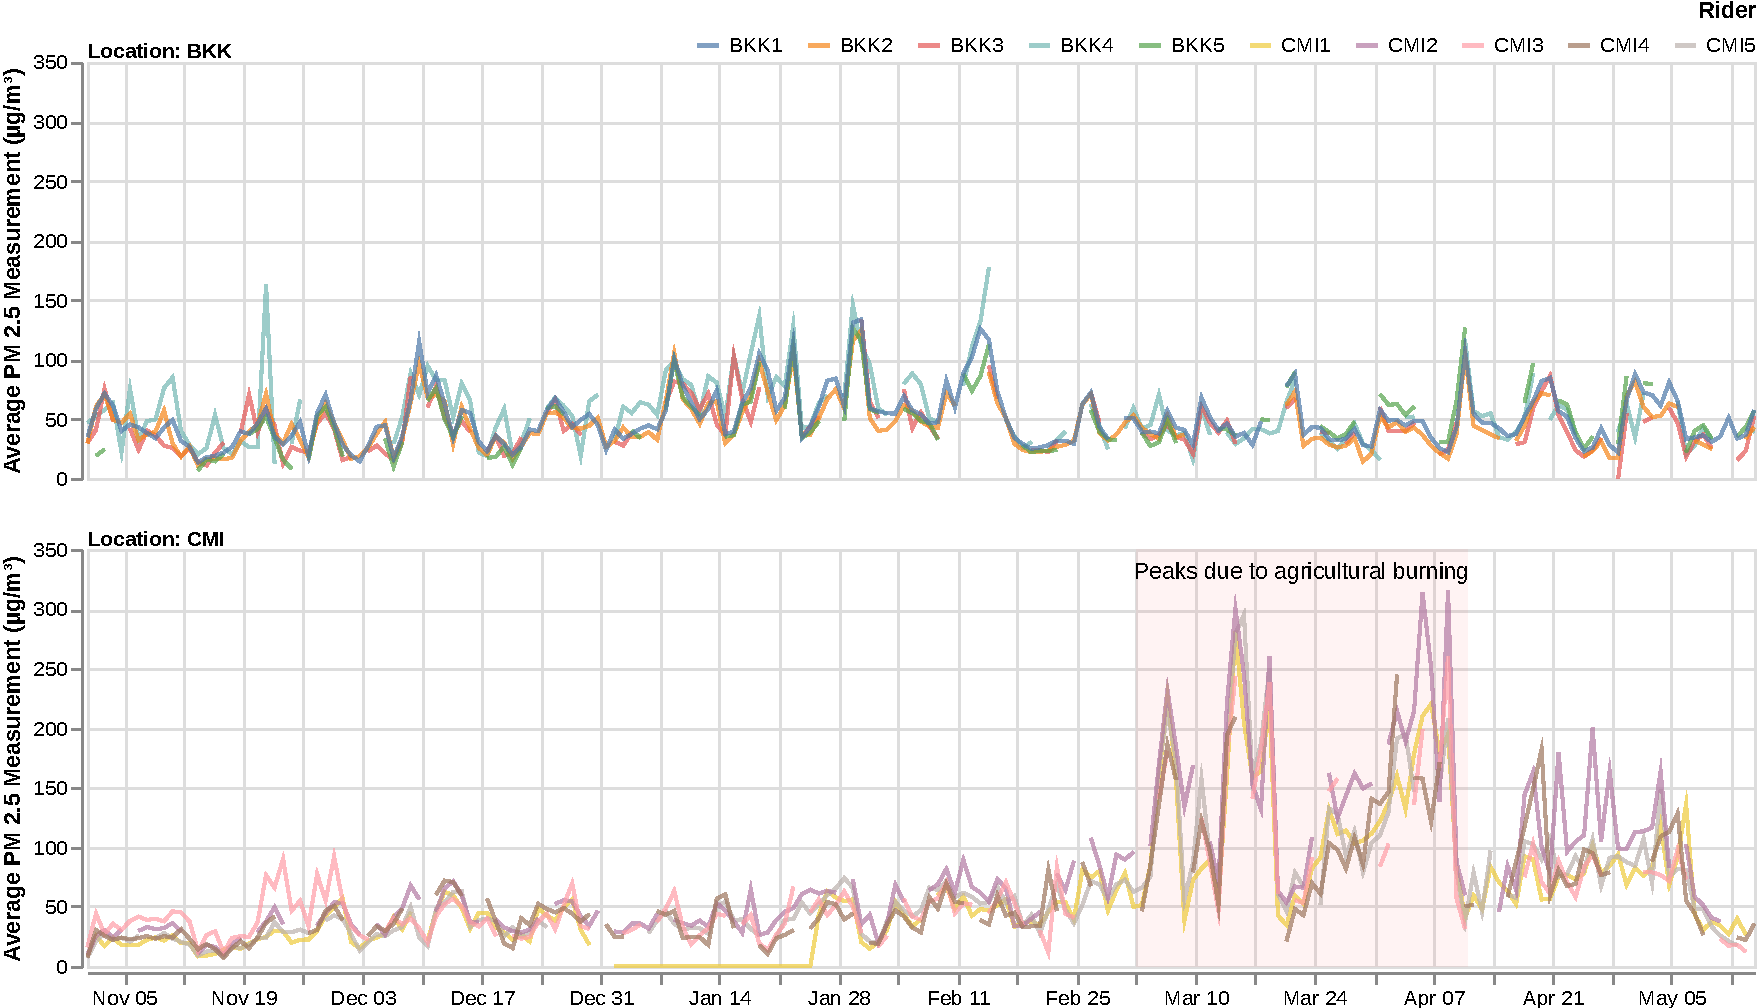
\includegraphics[width=\textwidth]{figures/daily-pollution-per-rider.pdf}
    \caption{
    Daily PM 2.5 exposure measured from the helmet-mounted sensors for Bangkok and Chiang Mai drivers.
    Vertical grid lines represent Sundays.
    }
    \Description{}
    \label{fig:daily-pollution-per-driver}
\end{figure*}

\subsection{PM2.5's Temporal Patterns}
Analyzing daily average PM2.5 exposure (\autoref{fig:daily-pollution-per-driver}) reveals relatively consistent levels in Bangkok (BKK), peaking moderately from December to mid-February,
while Chiang Mai (CMI) shows pronounced seasonality with extreme peaks from March to early April (consistent with agricultural burning periods~\cite{david2025chiangmaiburn, bernsten2024chiangmaiburn, iqair2023chiangmaiburn}).
% \joe{if you're going ot highlight it in the text like this, i would also highlight it in the figure}
Within each city, drivers experience similar daily trends.
Hourly averages (\autoref{fig:hourly-work-aqi}) show daily cycles peaking during morning (BKK: 7 AM, CMI: 8 AM) and evening rush hours, with an afternoon dip, although late night/early morning data shows higher variance.
Notably, BKK's PM2.5 measurements show a consistent trend throughout the year, reinforcing traffic as the primary air pollution source.
In contrast, CMI's dominant seasonal variation indicates agricultural burning as the primary driver.
Thus, PM2.5 sources differ substantially between cities (BKK: traffic, CMI: agricultural burning), implying the need for location-specific mitigation strategies.

% To find the PM 2.5 exposure amount of each driver throughout the different periods of the study,
% we present a relationship of the average amount of PM 2.5 measured from our sensor against days in the study in \autoref{fig:daily-pollution-per-driver}.
% We can see that the peak pollution in Bangkok is from December to mid-February; however, the amount of air pollution Bangkok drivers are exposed to is relatively consistent throughout the study period compared to that of Chiang Mai.
% On the other hand, PM 2.5 in Chiang Mai reaches high peaks from March to early April and low peaks afterward until May.
% We can attribute this consistency of the PM 2.5 level in Bangkok to its constant heavy traffic.
% In contrast, the condensed PM 2.5 peak period in Chiang Mai is consistent with yearly agricultural burning periods,
% which typically end in April,
% as evidenced by climate articles~\cite{david2025chiangmaiburn, bernsten2024chiangmaiburn, iqair2023chiangmaiburn}.
% % \mick{enforcement for agricultural burning}\footnote{\mick{\url{https://radiochiangmai.prd.go.th/th/content/category/detail/id/57/iid/352430}, \url{https://maesa.go.th/public/list/data/detail/id/5046/menu/1554}}}
% In addition, despite each driver's independence,
% all of the drivers in the study in each location still are exposed to the same amount of pollution, as shown in \autoref{fig:daily-pollution-per-driver}.

% To drill down into the finer-grain time period, we analyze PM 2.5 exposure patterns throughout each of the drivers' work days, as shown in \autoref{fig:hourly-work-aqi}.
% We can observe that the PM 2.5 exposure is consistently the highest at 7 AM for Bangkok and 8 AM for Chiang Mai, as these are both provinces' rush hours.
% The measurements for both provinces consistently slope down until the afternoon when they reach their lowest measurement values.
% The measurements climb back up again in the evening as workers travel back to their residents.
% The measurements collected at late night and early morning are inconsistent as indicated by the wider standard deviation range.
% % \mick{can we say here that because we have fewer data points -> less consistent?}
% The pattern with high PM 2.5 exposure during the morning and afternoon is less visible from March to May in Bangkok.
% This is the period when the majority of schools in Bangkok are on Summer break.
% The measured PM 2.5 patterns are highly correlated with Bangkok residents' commute behavior.
% This correlation further emphasizes that the primary source of PM 2.5 measured by Bangkok drivers is traffic pollution.
% On the other hand, in Chiang Mai, the measured PM 2.5 pattern with respect to months of the year is more prominent than patterns observed from measured PM 2.5 within a day.
% This indication leads us to conclude that the primary source of PM 2.5 measured by Chiang Mai drivers is agricultural burning.
% These results are also consistent with our analysis for \autoref{fig:daily-pollution-per-driver}.
% % \mick{can add analysis of PM 2.5 per day of the week if we have space.}

\begin{figure*}
    \centering
    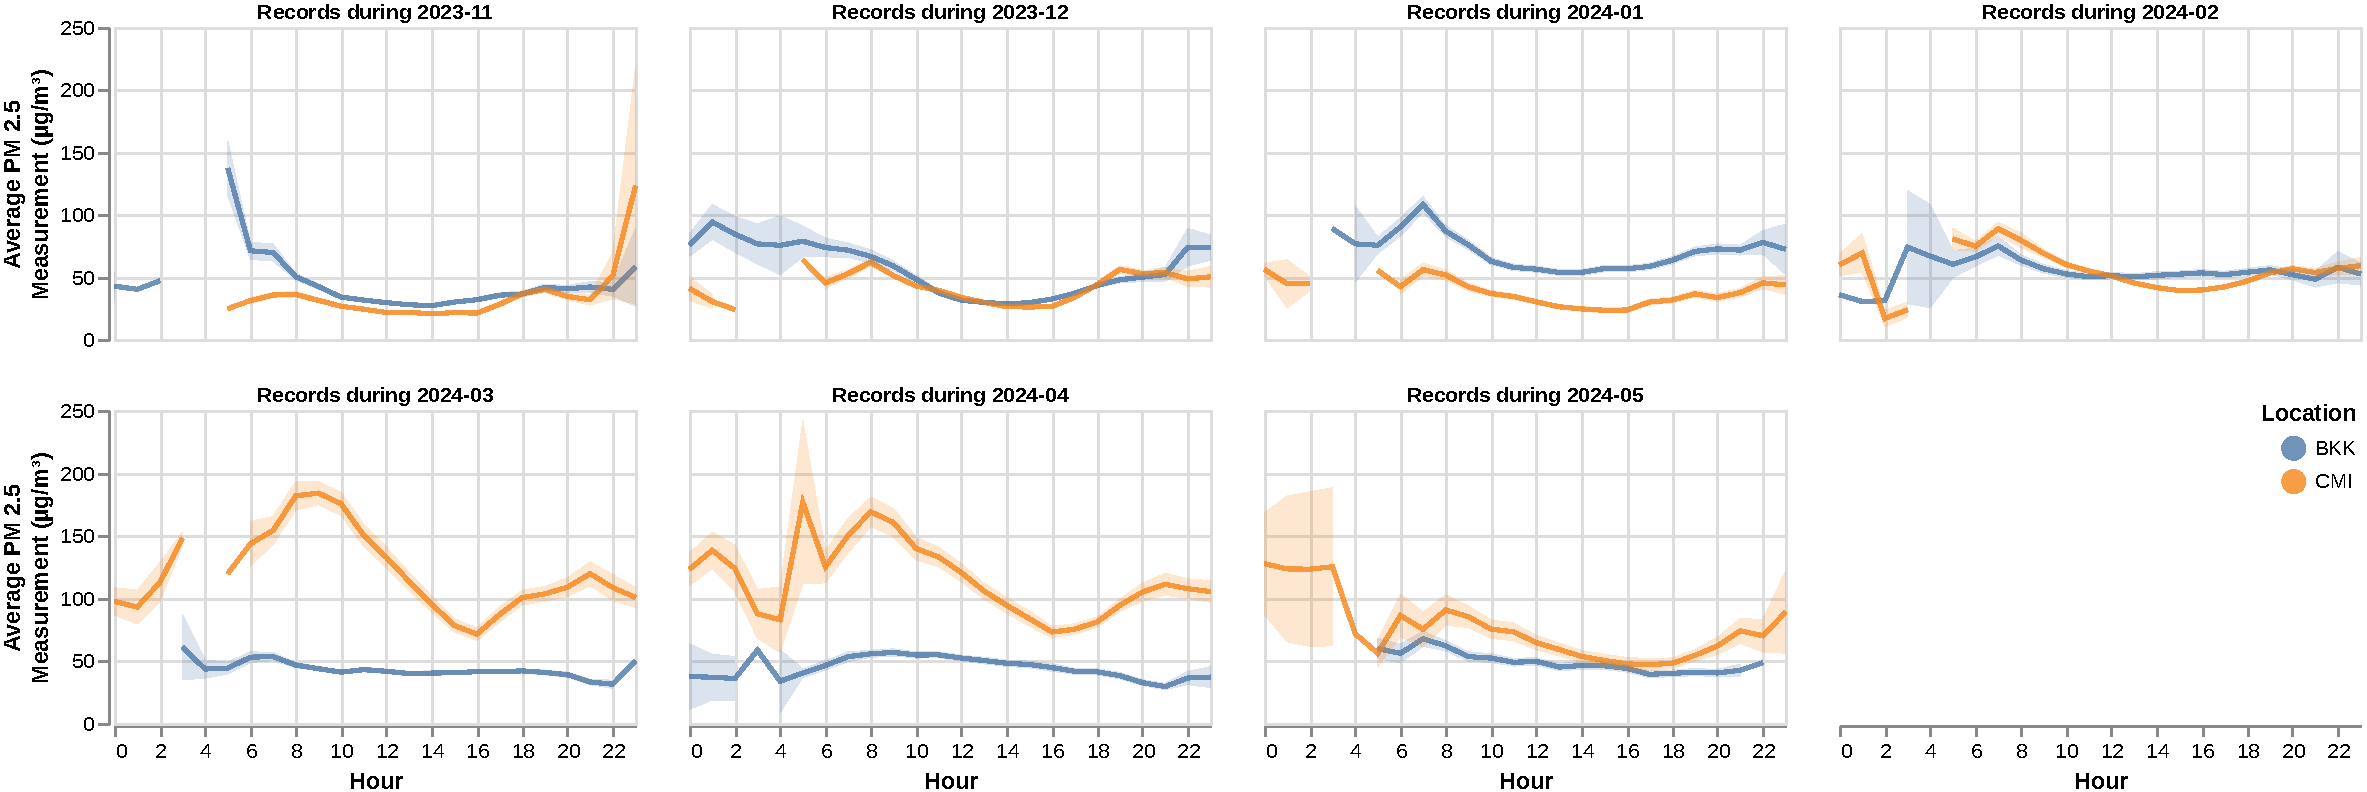
\includegraphics[width=\textwidth]{figures/average-hourly-pollution.pdf}%
    \caption{Mean and standard deviations of air pollution measurement in each hour of the day throughout the study period.
    % Each colored band represents $\pm1$ standard deviation from its average line. \joe{you can just say "mean and standard deviations shown" people know what fillbetween() represents.}
    Each subplot represents each month in the study. }%
    \Description{}
    \label{fig:hourly-work-aqi}%
\end{figure*}%

% % \begin{figure}
% %     \centering
% %     \begin{subfigure}[t]{0.49\textwidth}
% %         \centering
% %         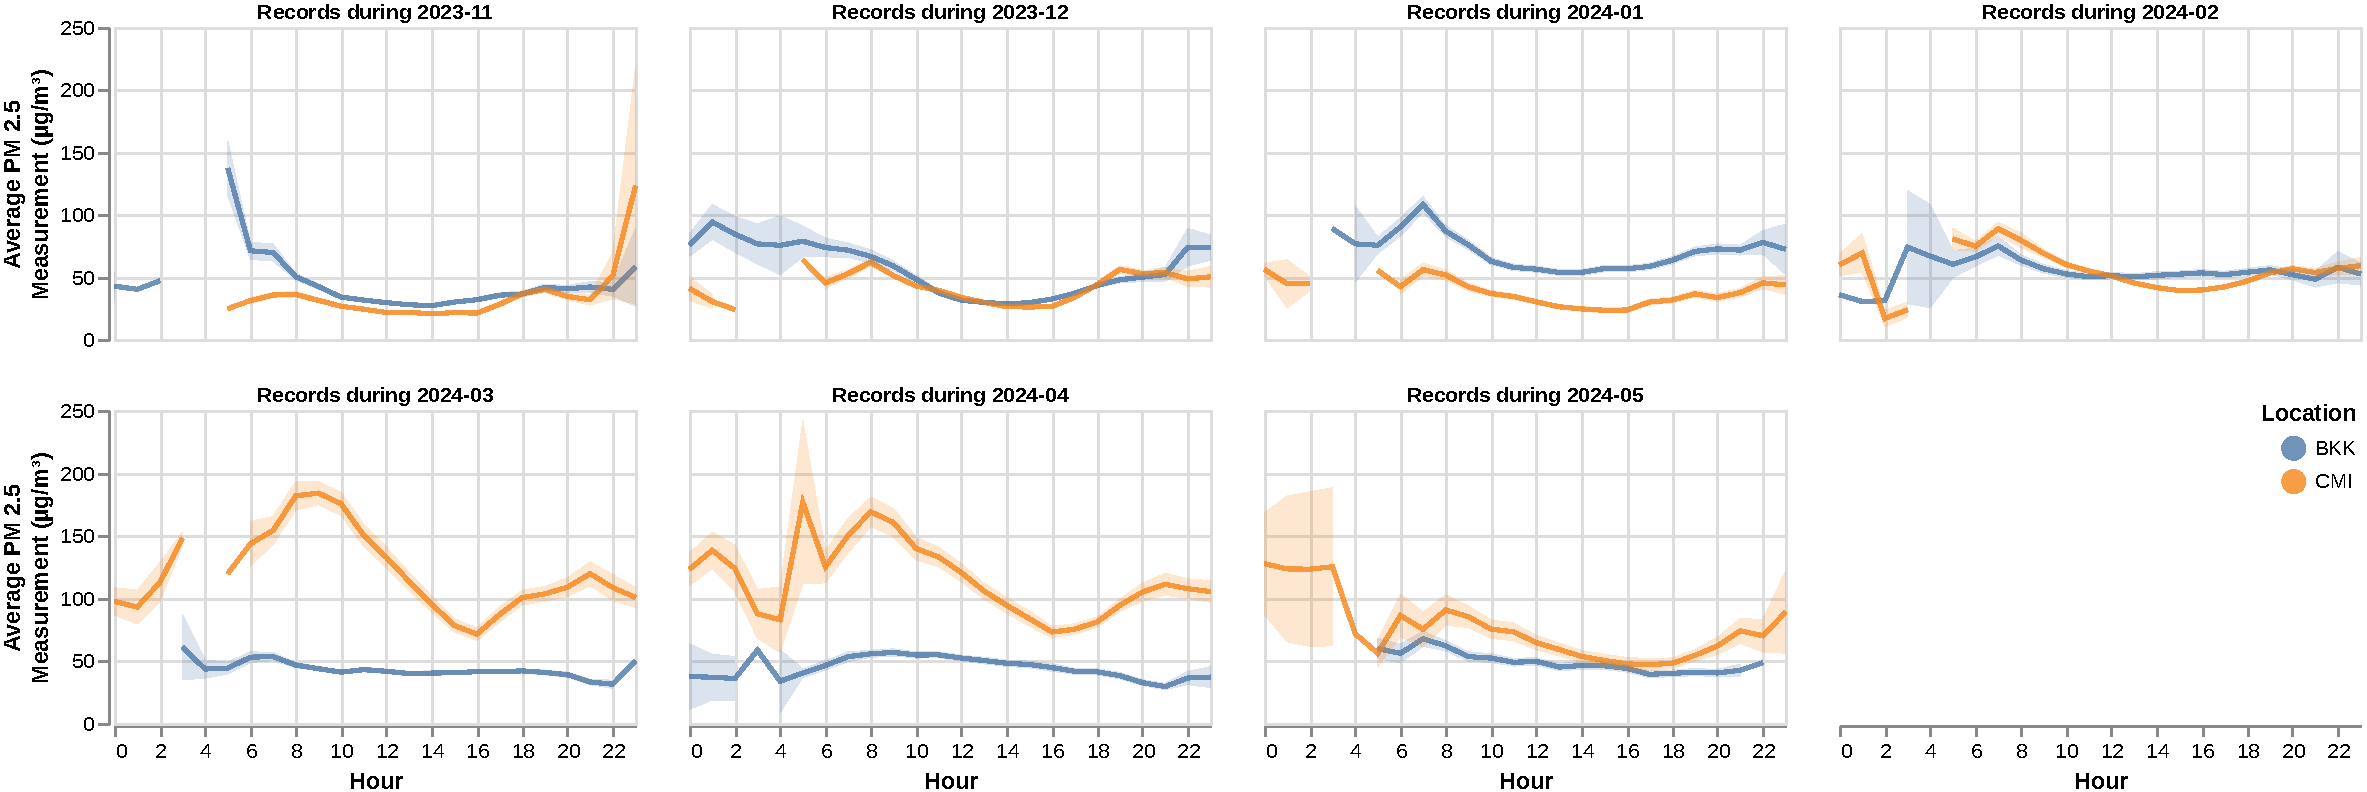
\includegraphics[width=\linewidth]{figures/average-hourly-pollution.pdf}%
% %         \caption{Average air pollution measurement in each hour of the day throughout the study period.}
% %         \label{fig:hourly-work-aqi}
% %     \end{subfigure}%
% %     \hfill%
% %     \begin{subfigure}[t]{0.49\textwidth}
% %         \centering
% %         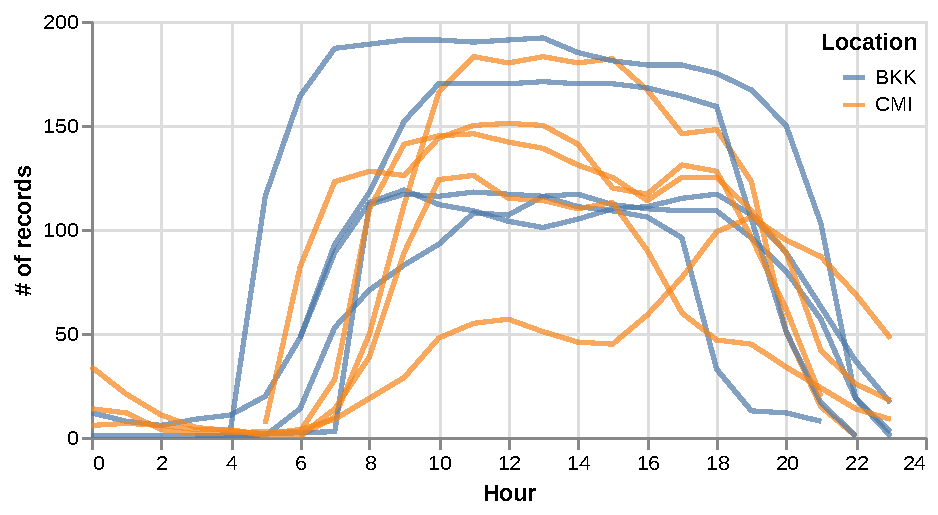
\includegraphics[width=\linewidth]{figures/hourly-records-per-location.pdf}%
% %         \caption{Number of records for each hour of the day throughout the study period. \mick{todo: divide by the \# of days they work}}
% %         \label{fig:hourly-work-hours}
% %     \end{subfigure}%
% %     \caption{
% %     Air pollution exposure and hour work for each hour of the day.
% %     \joe{shift x axis index by 1 so its not 0-23 but 1-24 for right plot and explain in text whether we actually have rider data from 22-3 as and how often. was it a few riders that drove at night?}
% %     }%
% %     \label{fig:hourly-work-stats}%
% % \end{figure}%

% % {\bf Answers to QS1.}
% \paragraph{Answers to QS1}
% % \mick{peaks at xxx; bkk is more consistent; chiang mai has lower pm 2.5 values during the normal period, but higher peaks; drivers seem to be exposed to similar amounts of PM 2.5 among drivers in the same province.}
% The PM 2.5 measured in Chiang Mai primarily follows the patterns of agricultural burning,
% while PM 2.5 measured in Bangkok primarily correlates with the commute behaviors of Bangkok residents and, thus, likely comes from traffic pollution.
% % \mick{the time granularity? for tackling AQ problem in each region are different (no one solution that fits regions)}
% As a result, the solution for lessening the amount of PM 2.5 exposed between both provinces must be different depending on the source of air pollution.

\subsection{PM2.5's Spatial Patterns}
% The results from analyzing the temporal patterns of PM 2.5 measurement indicate that participants in the same province are exposed to PM 2.5 at a similar amount at any given time throughout the study.
% In this section, we analyze the relationship between the amount of PM 2.5 measured and the locations of the drivers.
% As shown in \autoref{fig:subdistrict-aqi}, in each sub-figure, the plots in the right columns reveal that all of the drivers in the study mostly stay in one location. 
% The plots in the left columns also reveal that the PM 2.5 level is distributed unevenly across both provinces' subdistricts and drivers.

% \paragraph{Answer to QS2}
% The drivers experience different amounts of PM 2.5 even at the same approximate location.
% Each driver also spends the majority of their time at a different place.
% As a result, the solution for reducing the drivers' exposure to PM 2.5 should also take into account their active locations during their work.
Spatial analysis (\autoref{fig:subdistrict-aqi}) reveals that PM2.5 distribution is uneven across subdistricts and individual drivers, with drivers experiencing different exposure levels even in similar areas.
Furthermore, each driver tends to operate primarily within specific locations.
Consequently, effective PM2.5 exposure mitigation strategies must consider these individual spatial work patterns.
% \joe{is there openstreetmap in bangkok and chiangmai? can you compare the AQI with some environmental feature that you can pull from OSM? For example, number of intersections, width of roads, density of roads, etc. Would be cool to try to actually learn something about why AQI is worse in certain areas.}



\begin{figure*}[t]
    \centering

    % Bangkok
    \begin{subfigure}[t]{0.49\textwidth}
        \centering
        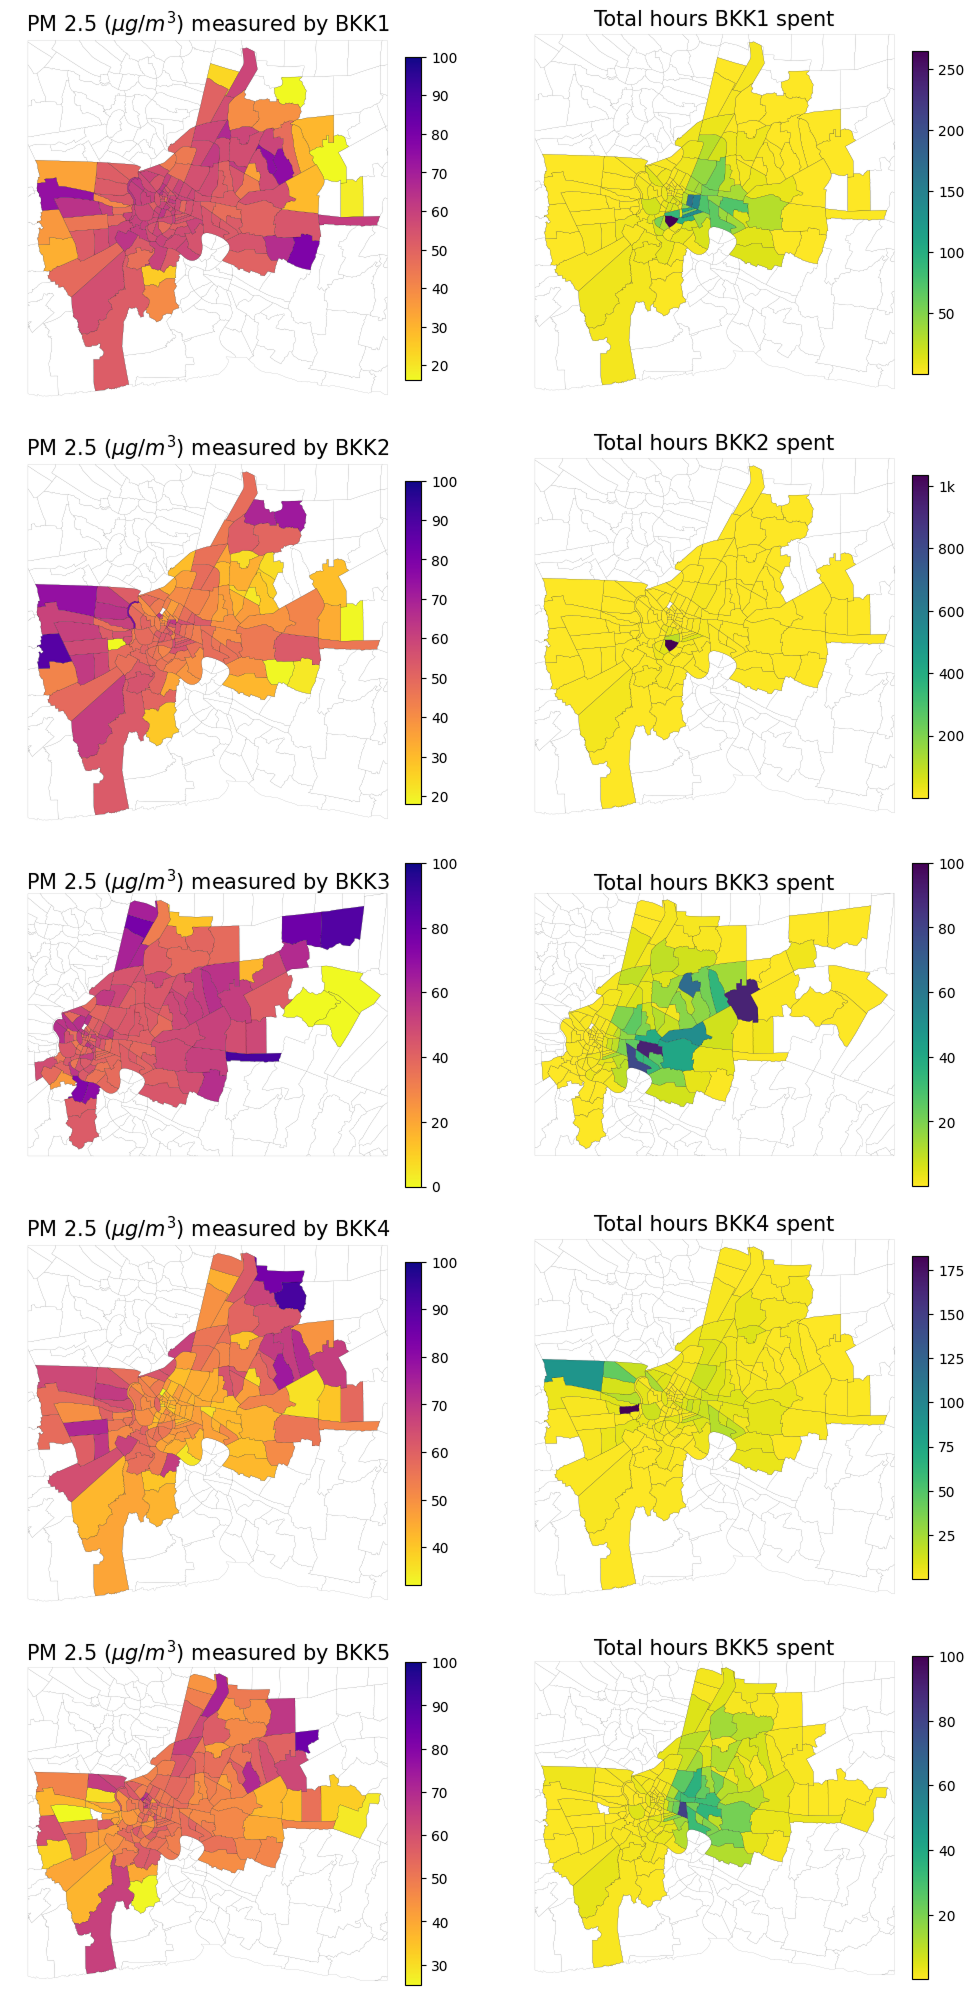
\includegraphics[width=\linewidth]{figures/map/BKK_PM_TIME.png}%
        % 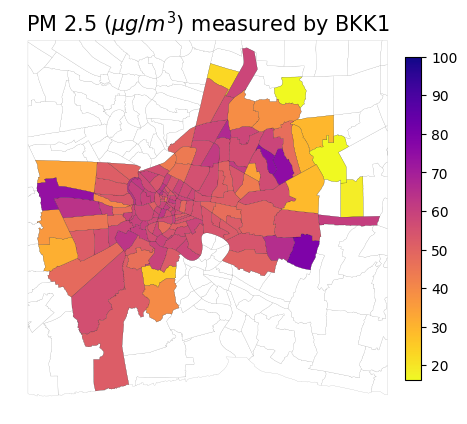
\includegraphics[width=.48\linewidth]{figures/map/BKK1_PM25.png}%
        % 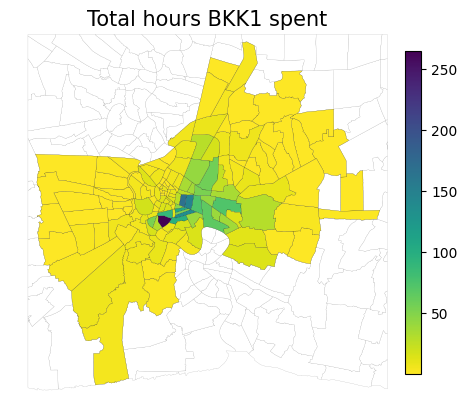
\includegraphics[width=.48\linewidth]{figures/map/BKK1_time.png}\\[0.3em]
        % 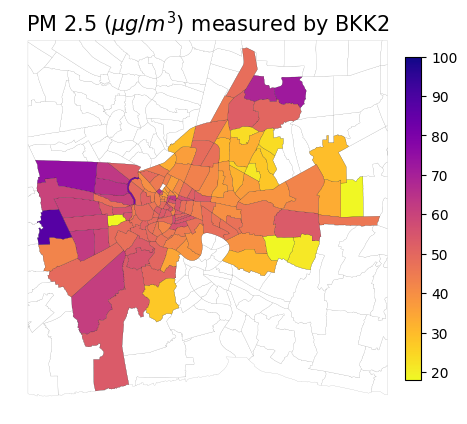
\includegraphics[width=.48\linewidth]{figures/map/BKK2_PM25.png}%
        % 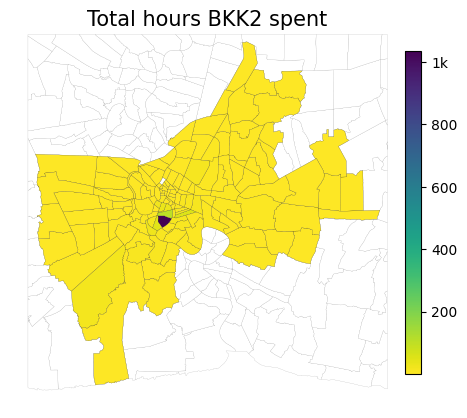
\includegraphics[width=.48\linewidth]{figures/map/BKK2_time.png}\\[0.3em]
        % 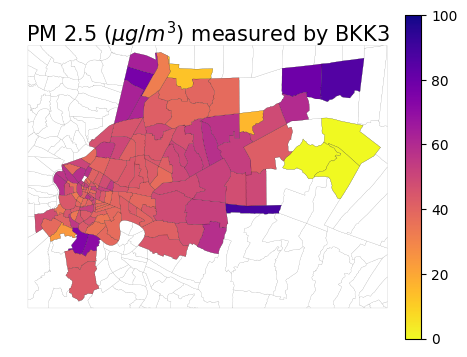
\includegraphics[width=.48\linewidth]{figures/map/BKK3_PM25.png}%
        % 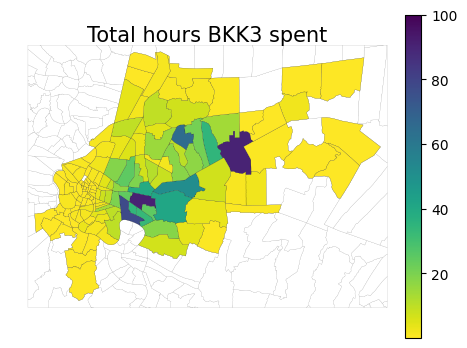
\includegraphics[width=.48\linewidth]{figures/map/BKK3_time.png}\\[0.3em]
        % 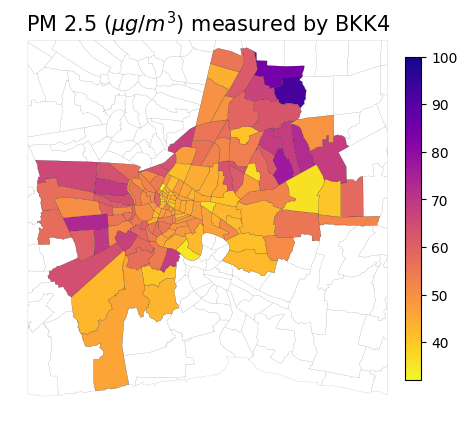
\includegraphics[width=.48\linewidth]{figures/map/BKK4_PM25.png}%
        % 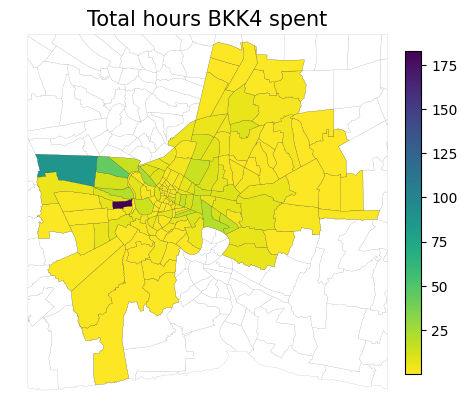
\includegraphics[width=.48\linewidth]{figures/map/BKK4_time.png}\\[0.3em]
        % 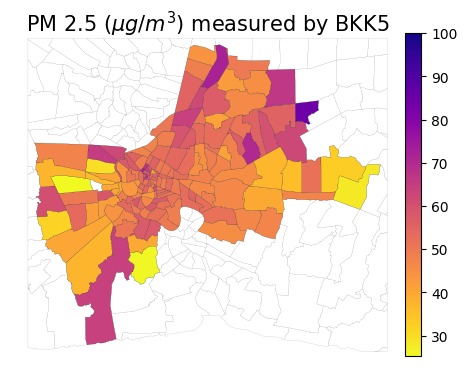
\includegraphics[width=.48\linewidth]{figures/map/BKK5_PM25.png}%
        % 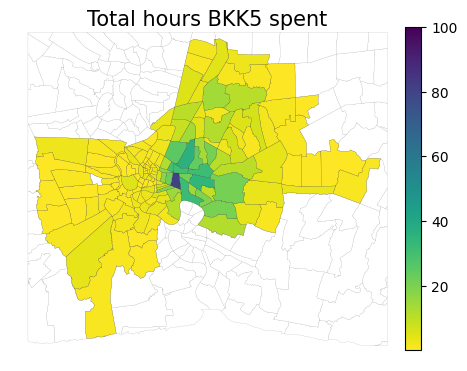
\includegraphics[width=.48\linewidth]{figures/map/BKK5_time.png}
        \caption{Measurement collected in Bangkok.}
    \end{subfigure}%
    \hfill
    % Chiang Mai
    \begin{subfigure}[t]{0.49\textwidth}
        \centering
        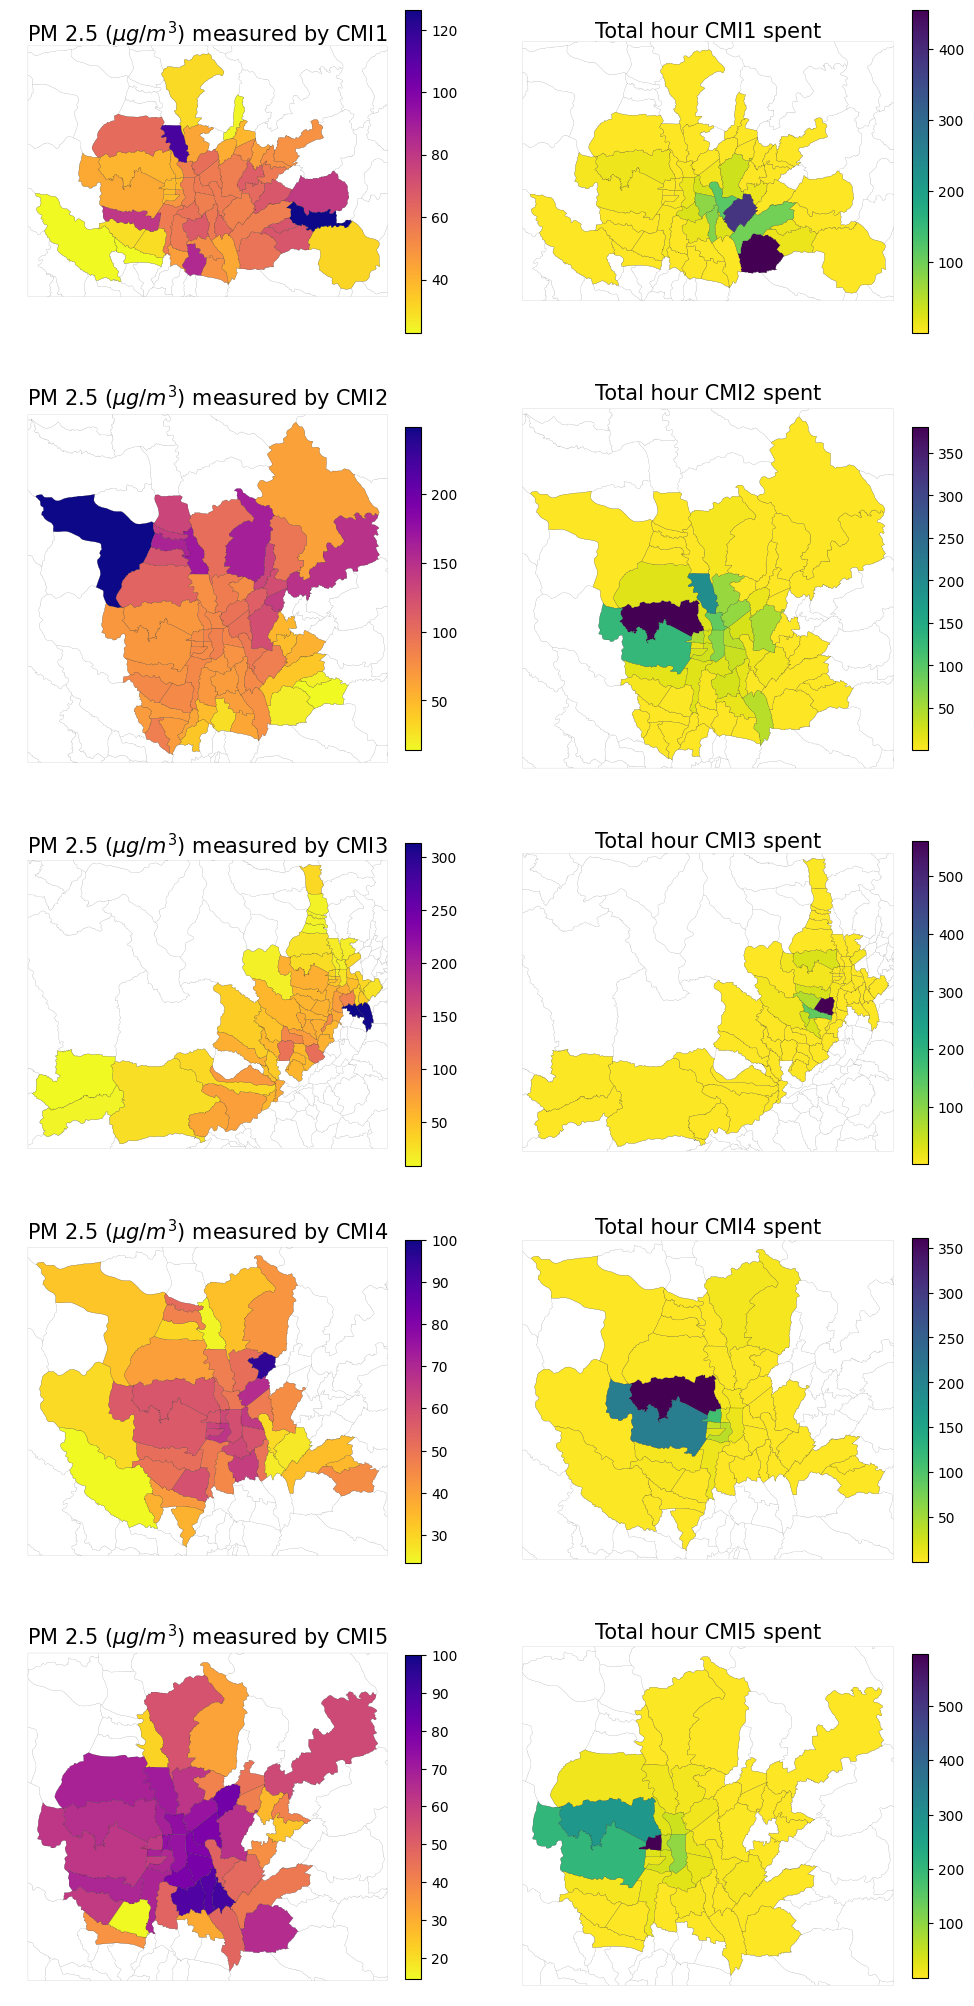
\includegraphics[width=\linewidth]{figures/map/CMI_PM_TIME.png}%
        % 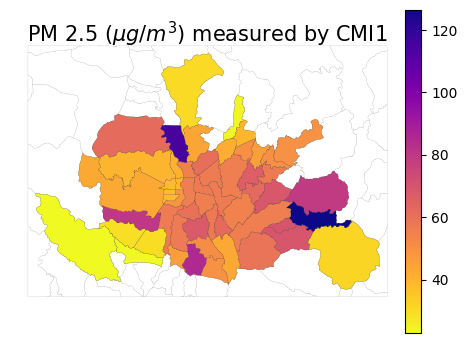
\includegraphics[width=.48\linewidth]{figures/map/CMI1_PM25.png}%
        % 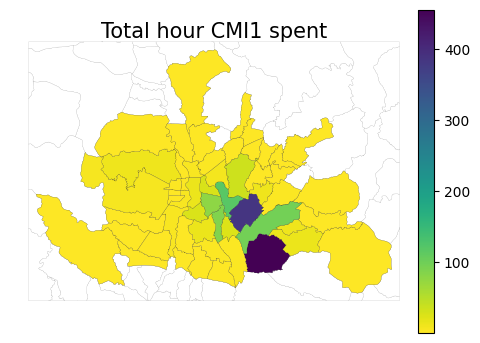
\includegraphics[width=.48\linewidth]{figures/map/CMI1_time.png}\\[0.3em]
        % 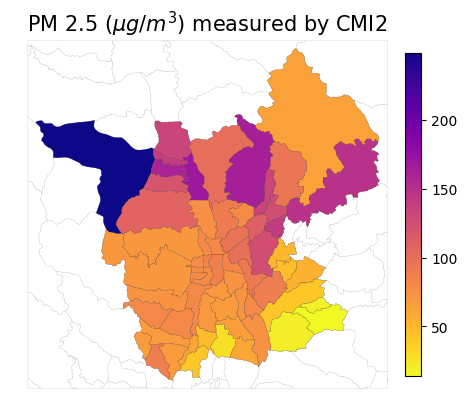
\includegraphics[width=.48\linewidth]{figures/map/CMI2_PM25.png}%
        % 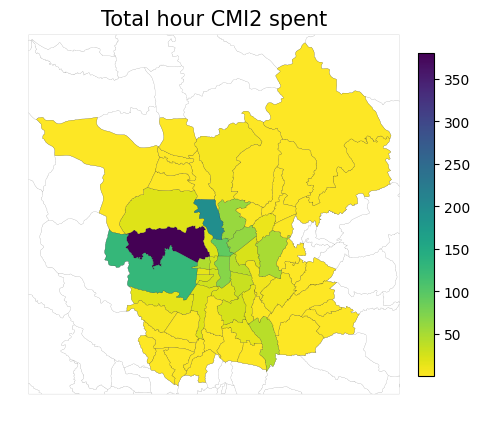
\includegraphics[width=.48\linewidth]{figures/map/CMI2_time.png}\\[0.3em]
        % 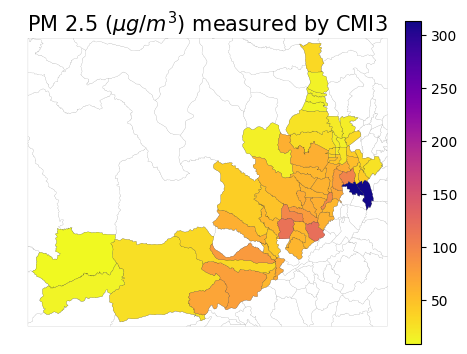
\includegraphics[width=.48\linewidth]{figures/map/CMI3_PM25.png}%
        % 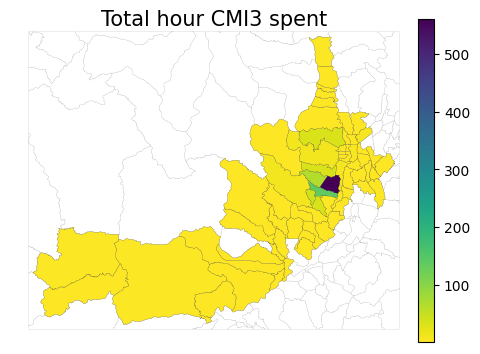
\includegraphics[width=.48\linewidth]{figures/map/CMI3_time.png}\\[0.3em]
        % 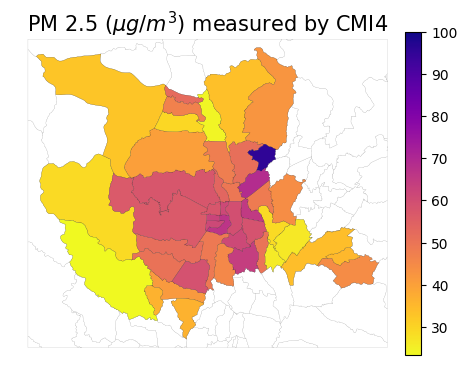
\includegraphics[width=.48\linewidth]{figures/map/CMI4_PM25.png}%
        % 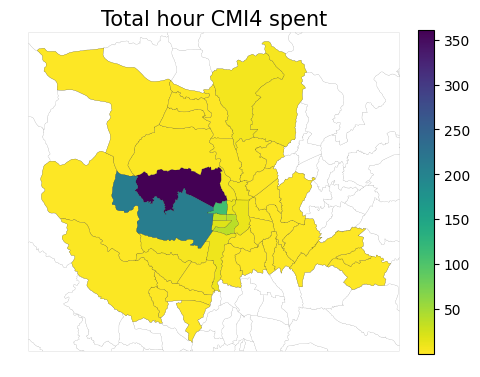
\includegraphics[width=.48\linewidth]{figures/map/CMI4_time.png}\\[0.3em]
        % 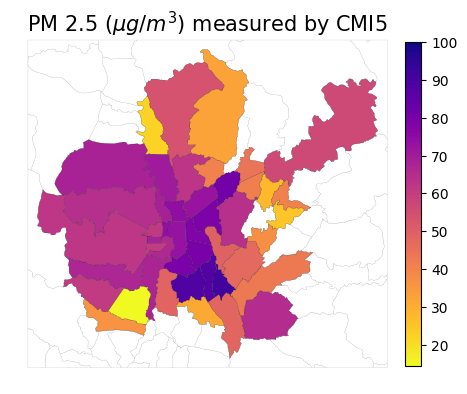
\includegraphics[width=.48\linewidth]{figures/map/CMI5_PM25.png}%
        % 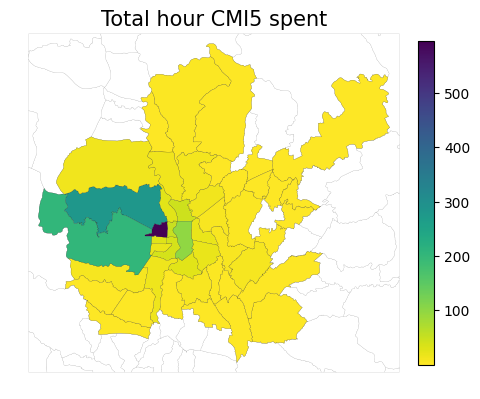
\includegraphics[width=.48\linewidth]{figures/map/CMI5_time.png}
        \caption{Measurement collected in Chiang Mai.}
    \end{subfigure}%

    \caption{
    The left column of each sub-figure shows the average PM2.5 level throughout the study period measured in each subdistrict.
    The right column of each sub-figure shows the amount of time in hours that each driver spent in each subdistrict throughout the study.
    }
    \Description{}
    \label{fig:subdistrict-aqi}
\end{figure*}


% \begin{figure*}[t]
%     \centering
%     \begin{subfigure}[t]{0.49\textwidth}
%         \centering
%         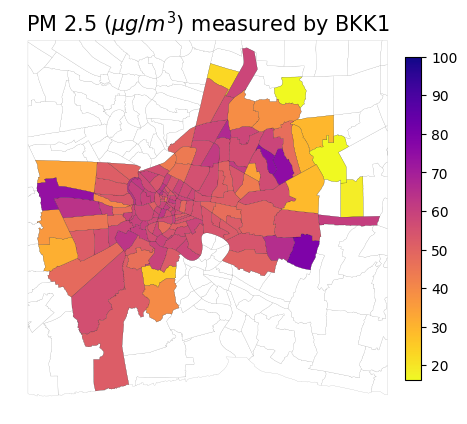
\includegraphics[width=.49\linewidth]{figures/map/BKK1_PM25.png}%
%         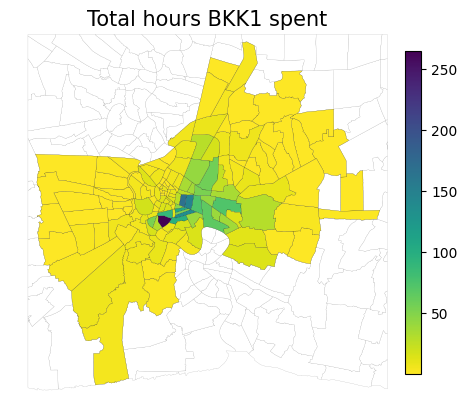
\includegraphics[width=.49\linewidth]{figures/map/BKK1_time.png}
%         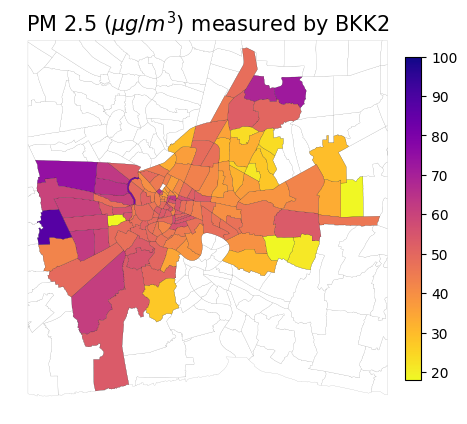
\includegraphics[width=.49\linewidth]{figures/map/BKK2_PM25.png}%
%         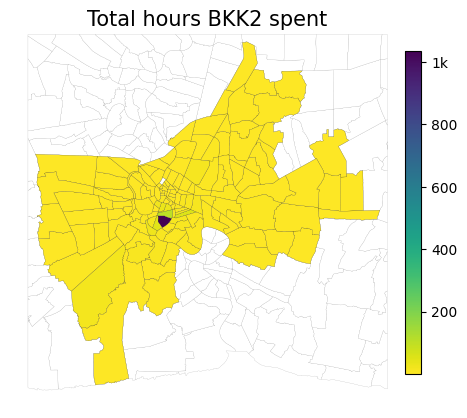
\includegraphics[width=.49\linewidth]{figures/map/BKK2_time.png}
%         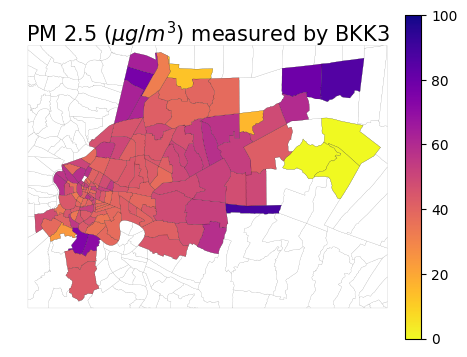
\includegraphics[width=.49\linewidth]{figures/map/BKK3_PM25.png}%
%         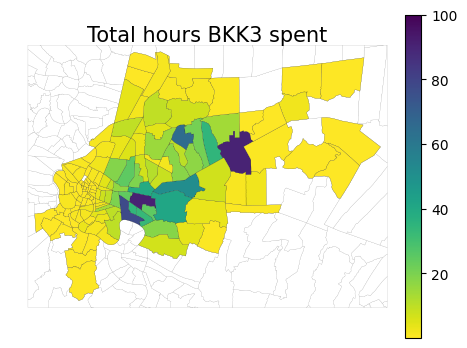
\includegraphics[width=.49\linewidth]{figures/map/BKK3_time.png}
%         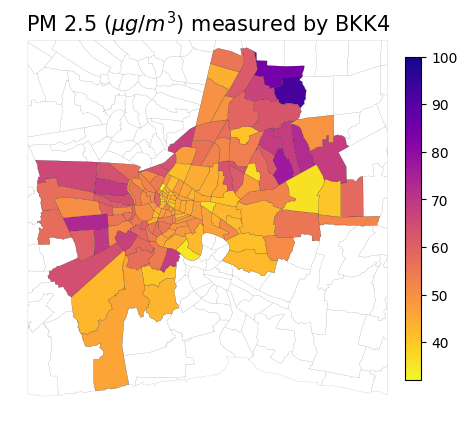
\includegraphics[width=.49\linewidth]{figures/map/BKK4_PM25.png}%
%         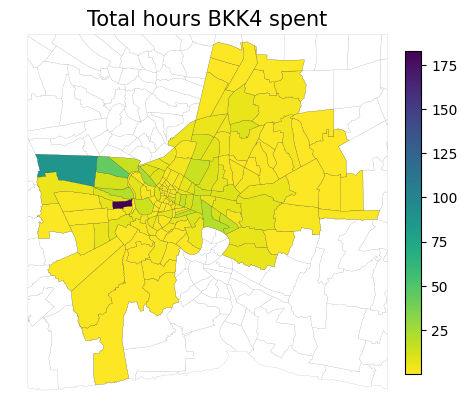
\includegraphics[width=.49\linewidth]{figures/map/BKK4_time.png}
%         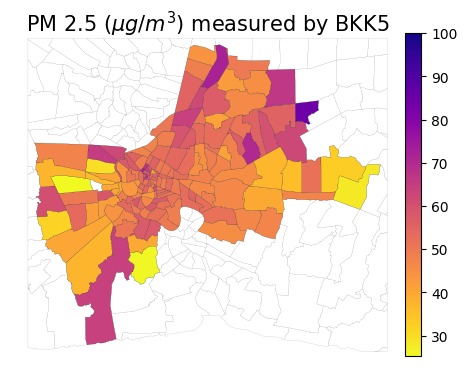
\includegraphics[width=.49\linewidth]{figures/map/BKK5_PM25.png}%
%         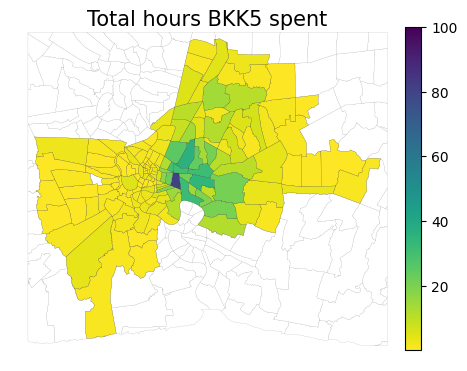
\includegraphics[width=.49\linewidth]{figures/map/BKK5_time.png}
%         \caption{Measurement collected in Bangkok.}
%         % \label{fig:hourly-work-aqi}
%     \end{subfigure}%
%     \hfill%
%     \begin{subfigure}[t]{0.49\textwidth}
%         \centering
%         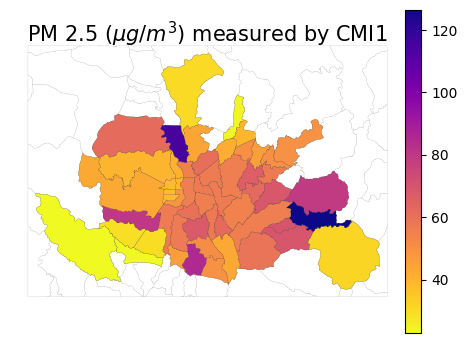
\includegraphics[width=.49\linewidth]{figures/map/CMI1_PM25.png}%
%         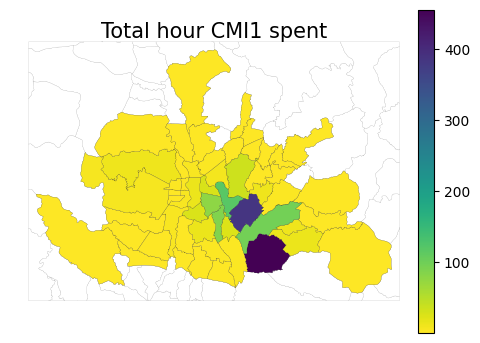
\includegraphics[width=.49\linewidth]{figures/map/CMI1_time.png}
%         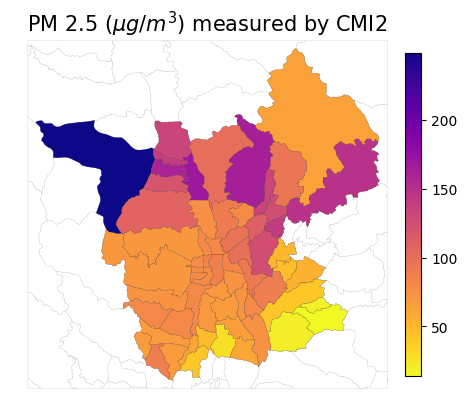
\includegraphics[width=.49\linewidth]{figures/map/CMI2_PM25.png}%
%         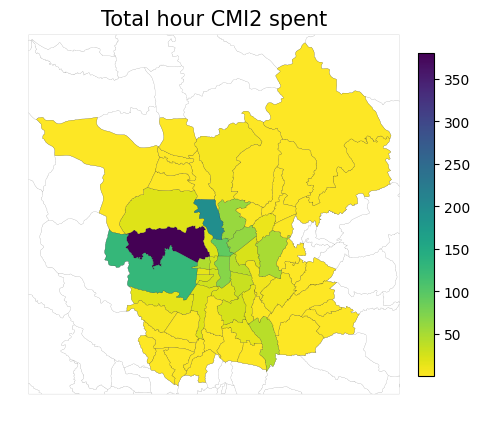
\includegraphics[width=.49\linewidth]{figures/map/CMI2_time.png}
%         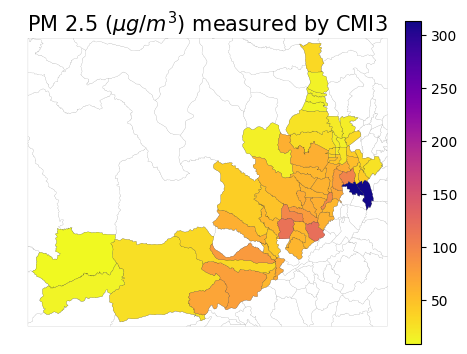
\includegraphics[width=.49\linewidth]{figures/map/CMI3_PM25.png}%
%         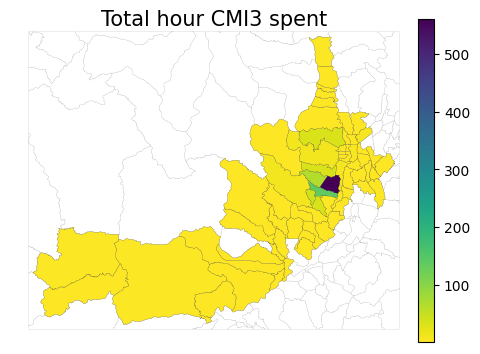
\includegraphics[width=.49\linewidth]{figures/map/CMI3_time.png}
%         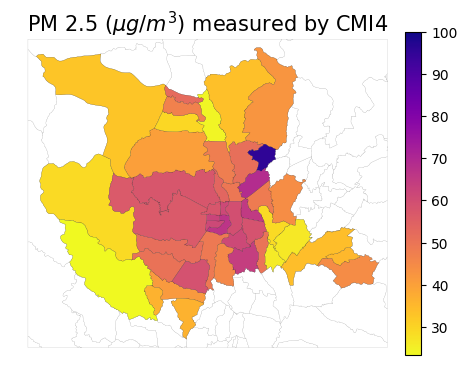
\includegraphics[width=.49\linewidth]{figures/map/CMI4_PM25.png}%
%         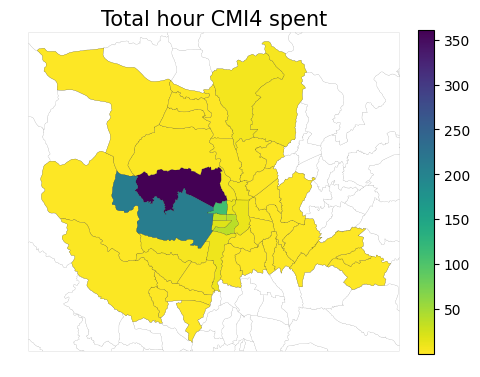
\includegraphics[width=.49\linewidth]{figures/map/CMI4_time.png}
%         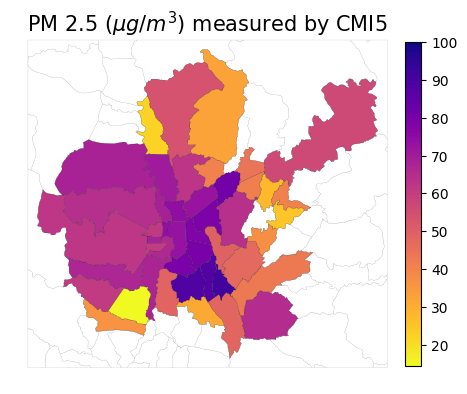
\includegraphics[width=.49\linewidth]{figures/map/CMI5_PM25.png}%
%         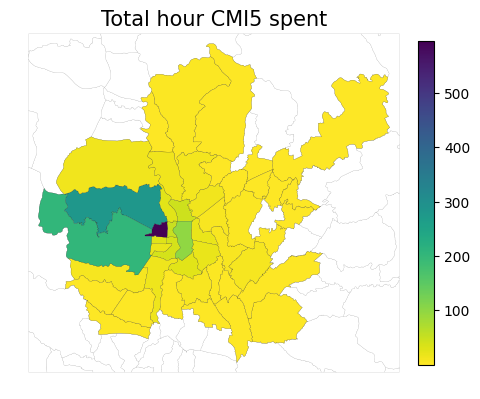
\includegraphics[width=.49\linewidth]{figures/map/CMI5_time.png}
%         \caption{Measurement collected in Chiang Mai.}
%         % \label{fig:hourly-work-hours}
%     \end{subfigure}%
%     \caption{
%     % \joe{wait... the color bars are all wildly different on these plots lol. you can't even compare between them...}
%     The left column of each sub-figure shows the average PM2.5 level throughout the study period measured in each subdistrict.
%     The right column of each sub-figure shows the amount of time in hours that each driver spent in each subdistrict throughout the study.
%     % \mick{todo: shared color axis?}
%     % \mick{todo: same vis sizes}
%     % \mick{todo: use latex notation for units}
%     % \mick{todo: include all the subdistricts}
%     % \joe{Shall we lower the opacity of the districts where there is no data at all in the left plots? based on the right plot, I can't tell if the purple districts have 0 hours spent or a very small amount of hours spent. If it is 0, I don't want to see measurements in the left plot. Maybe every person spent time in every district so if we want to make this more clear, just do a log plot in color dimension.}
%     }%
%     \Description{}
%     \label{fig:subdistrict-aqi}%
% \end{figure*}%
 